% Summary of the thesis (max 3 pages), separate document.
% Figures: ../images (thesis) and figures/ (made by Code/figure_summary/*.py).
% Build: cd summary && latexmk -pdf -interaction=nonstopmode summary.tex
\documentclass[11pt,a4paper]{article}
\usepackage[T1]{fontenc}
\usepackage[utf8]{inputenc}
\usepackage{lmodern}
\usepackage[hmargin=1.8cm,top=1.5cm,bottom=1.8cm]{geometry}
\usepackage{microtype}
\usepackage{graphicx}
\usepackage{booktabs}
\usepackage{amsmath}
\usepackage[font=small,labelfont=bf]{caption}
\usepackage[hidelinks]{hyperref}
\graphicspath{{figures/}{../images/}}
\captionsetup{skip=4pt}
\setlength{\parskip}{0pt}
\setlength{\textfloatsep}{8pt plus 2pt minus 2pt}
\setlength{\intextsep}{6pt plus 2pt minus 2pt}
\setlength{\floatsep}{8pt plus 2pt minus 2pt}
\pagestyle{plain}

\makeatletter
\renewcommand\section{\@startsection{section}{1}{\z@}{-1.4ex plus -0.5ex minus -0.2ex}{0.6ex plus 0.2ex}{\normalfont\large\bfseries}}
\makeatother

\begin{document}

\begin{center}
{\large\bfseries Vision-Based Row Following Navigation for Horticultural Robots\\with Automatically Labeled Semantic Segmentation\par}
\vspace{0.4em}
{Emanuele Pruiti\par}
\end{center}

\section{Introduction}

The shortage of skilled labor and the rising cost of farm management push agriculture towards autonomous robots, and row crops are among their most studied applications. A robot between two crop rows must stay in the corridor without damaging the plants, and satellite positioning alone is not enough for this. Dense canopies obstruct the GNSS signal and cause multi-path reflections, greenhouse structures also obstruct it, and GNSS with RTK corrections and 3D LiDAR are costly. A monocular RGB camera is a cost-effective alternative. Classical camera pipelines isolate the plants with color indices and thresholds, which break with changes of light, shadows and weeds. Segmentation networks handle these conditions better, but they need many images annotated by hand at pixel level and must run fast on the onboard computer.

Our solution guides the robot with the color images of one camera, without a map of the field. For each frame (Figure~\ref{fig:pipeline}), an LR-ASPP network predicts a mask of the path, the corridor between the rows. A centerline extractor turns this mask into a straight centerline, and a proportional controller steers the robot to keep the centerline at the center of the image. Segmenting first is also the idea behind EdgeNet. A network that found the centerline directly in the camera images would need images with the centerline marked by hand. EdgeNet finds it in the mask, so it can be trained on generated masks whose centerline is known exactly, and with it no stage of the chain needs manual annotation. The work has three parts:
\begin{enumerate}\setlength{\itemsep}{0pt}
\item the network is trained only on automatic labels, generated offline by SAM~3 from text prompts without manual correction, and these labels are compared with manual labels on lettuce images,
\item two extractors, Strip-IRLS and EdgeNet, are compared offline with three baselines,
\item the complete chain runs on the robot Demetra and was tested in a crop row with all five extractors, to see whether the network trained only on automatic labels, and the whole pipeline, can guide the robot along the row.
\end{enumerate}

\begin{figure}[h]
  \centering
  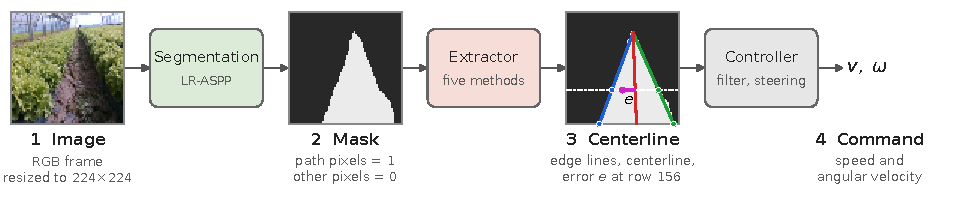
\includegraphics[width=0.75\linewidth]{pipeline_summary.pdf}
  \caption{Steps that run on the robot for each camera frame. The extractor turns the path mask into the two edge lines and the centerline, and the controller reads the lateral error $e$ at row 156 of the $224\times224$ mask.}
  \label{fig:pipeline}
\end{figure}

\section{Segmentation trained on automatic labels}

The images were recorded in a commercial greenhouse with the camera of the robot: 762 of lettuce, 878 of tomato and 319 of cucumber. Manual masks were drawn only for the lettuce images, because annotation is time-consuming.

FCN, DeepLabV3 and LR-ASPP were fine-tuned from pretrained TorchVision weights on the manual lettuce masks, with four classes. FCN and DeepLabV3 reach an mIoU of 0.9253, 1.08 percentage points above LR-ASPP, while LR-ASPP is 7.2 times faster than FCN and 10.6 times faster than DeepLabV3 on the training GPU. With a similar accuracy, speed decided, because the network runs on the robot in real time, and LR-ASPP was chosen.

The automatic labels were generated offline by SAM~3, with one text prompt per class such as \texttt{central farm path}, and were used for training without inspection or correction. Networks trained on automatic labels with four, three and two classes were compared with the network trained on manual masks, on the same 77 lettuce test images. On all 77 images, the path IoU of the automatic-label networks is only 0.39 to 0.41. The other 35 images show more than one path or were taken outside the rows. There the manual mask marks only the path to follow, while the automatic-label networks also mark the adjacent paths and the soil outside the corridor (Figure~\ref{fig:segmentation}a, bottom row). On the 42 test images taken between parallel rows, from viewpoints the robot can reach, the path IoU is 0.897 to 0.901, against 0.959 for the network trained on manual labels, 5.7 to 6.2 percentage points lower. The automatic labels are poor for the covering material (IoU of 0.17 against 0.83 on all 77 images), so they do not replace manual labels for every class. For the path between parallel rows, the four-, three- and two-class networks differ by less than 0.5 percentage points, and the robot uses a binary network, since the extractors need only the path.

The robot network, which tests this approach on the robot, is a binary LR-ASPP trained only on the automatic labels of all 1959 images. A copy trained without the 77 lettuce test images reaches a path IoU of 0.907 between parallel rows. Figure~\ref{fig:segmentation}b shows its output on tomato and cucumber.

\begin{figure}[h]
  \centering
  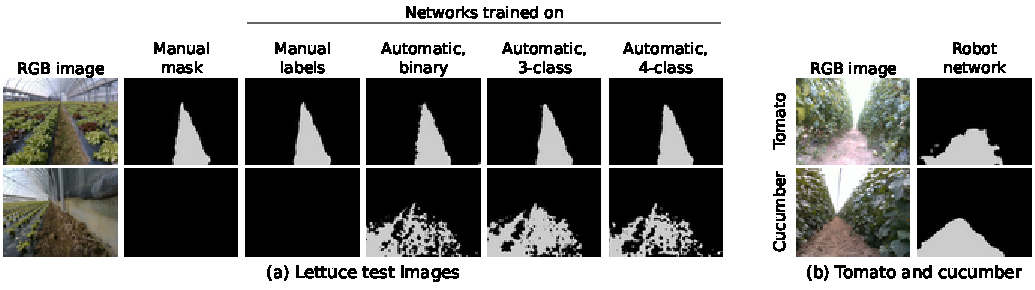
\includegraphics[width=0.85\linewidth]{segmentation_summary.pdf}
  \caption{Path masks. (a)~Lettuce test images with the manual mask and the output of the LR-ASPP networks trained on manual labels and on automatic labels with two, three and four classes. In the bottom image the automatic-label networks also mark the strips beside the corridor. (b)~Output of the robot network on tomato and cucumber images, which have no manual mask.}
  \label{fig:segmentation}
\end{figure}

\section{Extraction of the centerline}

All five extractors take the same $224\times224$ path mask and return a straight centerline, a confidence and a status, \texttt{ok}, \texttt{degraded} or \texttt{lost}. Strip-IRLS divides the lower part of the mask into horizontal strips and extracts the path intervals of each strip. Going up from the bottom of the image, it links in each strip the interval that continues the corridor found below, and it keeps the chain that gives the most edge samples. It then fits the left and right edges separately with iteratively reweighted least squares, and the centerline is the mean of the two lines. EdgeNet, still at an early stage, is a small network of about 0.8 million parameters that regresses the two corridor edges directly from the mask. Since it works on the mask and not on the camera image, it is trained only on generated masks, with errors like those of the segmentation, such as holes and blobs, and with exact edges, so it needs no manual annotation. Apart from the confidence thresholds that decide the status, it has no parameters to set by hand. The baselines are Center points (one line through the midpoints of the intervals), Column histogram (the column with the most path pixels) and RANSAC edges (the two edges fitted with RANSAC on the row extremes of the corridor).

The extractors were tested on 2400 synthetic masks with an exact centerline and on 255 real frames whose corridor edges were marked by hand. There is no clear winner, and finding one was not the aim. The tests show how the extractors behave in the different scenarios and which scenarios cause them the most problems (Table~\ref{tab:summary}). On the masks with one corridor and on the real frames, Strip-IRLS, EdgeNet and RANSAC edges have few gross errors, and these tests do not rank them. On the Jetson, Strip-IRLS is 1.4 times and EdgeNet 3.3 times faster than RANSAC edges. Adjacent corridors, outside the aim of this work, are the hardest synthetic case for RANSAC edges, with 24.7\% of gross errors against 3.0\% for Strip-IRLS. On the real frames, the 22 gross errors of the three best extractors fall on only 15 different frames, mostly of tomato, where the segmentation is much worse than on the others.

\begin{table}[h]
  \centering
  \footnotesize
  \caption{Results of the five extractors. Offline: a gross error is a centerline error above 15~px at the row read by the controller, and a \texttt{lost} frame has a corridor but no valid centerline, both in \% of the masks. Field: lateral distance of the robot from the row centerline. RMSE: mean of the three short runs, or the full-row run. Std runs: how much the three short runs differ at the same positions. RMSD: how much the mean of the short runs differs from that of the other four extractors.}
  \label{tab:summary}
  \setlength{\tabcolsep}{4pt}
  \begin{tabular}{@{}lccccc@{}}
    \toprule
     & \shortstack{Strip-IRLS\\(ours)} & \shortstack{EdgeNet\\(ours)} & \shortstack{RANSAC\\edges} & \shortstack{Center\\points} & \shortstack{Column\\histogram} \\
    \midrule
    \multicolumn{6}{@{}l}{\textit{Offline, synthetic masks}} \\
    One corridor (1900 masks): gross errors (\%) ($\downarrow$) & 0.3 & 0.1 & 0.1 & 1.8 & 23.0 \\
    Adjacent corridors (300 masks): gross errors (\%) ($\downarrow$) & 3.0 & 0.0 & 24.7 & 1.3 & 23.7 \\
    \multicolumn{6}{@{}l}{\textit{Offline, real frames with hand-marked edges (255)}} \\
    Gross errors (\%) ($\downarrow$) & 2.4 & 4.7 & 1.6 & 4.3 & 14.9 \\
    \texttt{lost} frames (\%) ($\downarrow$) & 2.0 & 0.8 & 2.0 & 13.7 & 5.5 \\
    \textit{On the robot:} time on the Jetson AGX Orin (ms) ($\downarrow$) & 11.07 & 4.68 & 15.52 & 7.27 & 0.91 \\
    \multicolumn{6}{@{}l}{\textit{Field tests}} \\
    Short runs: RMSE (cm) ($\downarrow$) & 5.7 & 5.3 & 5.4 & 5.7 & 5.5 \\
    Short runs: Std runs (cm) ($\downarrow$) & 0.6 & 0.3 & 0.6 & 0.4 & 4.3 \\
    Short runs: RMSD (cm) & 1.5 & 1.1 & 1.8 & 1.6 & 5.1 \\
    Full row: RMSE (cm) ($\downarrow$) & 9.1 & 8.4 & 9.4 & 9.2 & 8.5 \\
    \bottomrule
  \end{tabular}
\end{table}

\section{Tests on the robot}

Demetra, the four-wheel-steering robot of the tests, has an NVIDIA Jetson AGX Orin as onboard computer. Without the debug video, the whole processing of a frame takes 11.3 to 26.2~ms depending on the extractor, less than the 33.3~ms frame period of the camera, so every frame is processed.

The field tests were made on 4 November 2026 in a tomato row of a tunnel greenhouse, a field not present in the training data of the robot network, with sparse plants and poor light. The trajectory of the robot was measured with a total station. Each extractor made three short runs at 0.20~m/s, compared between 12 and 4~m from the station, and one run along the full row at 0.50~m/s, compared from 15 to 39~m. Between runs only the extractor changed. The row centerline passes through five points placed by eye on the center of the row, so it is not accurate to the centimeter.

The robot followed the row with all five extractors (Figure~\ref{fig:field}). The RMSE from the row centerline is 5.3 to 5.7~cm on the short runs and 8.4 to 9.4~cm on the full row, and the largest distance 13.6 and 20.4~cm. Strip-IRLS, EdgeNet, RANSAC edges and Center points drove the robot along almost the same trajectory, with an RMSD of 1.1 to 1.9~cm and a standard deviation between runs of 0.3 to 0.6~cm. Most of their RMSE is therefore a lateral distance common to all their runs, at the same positions along the row. It comes from the row itself, where the plants reach into the path or the predicted path widens, and from small errors of the row centerline, so these runs do not show which extractor is better. Column histogram is the exception, since its three short runs follow different curves, with a standard deviation between runs of 4.3~cm.

\begin{figure}[h]
  \centering
  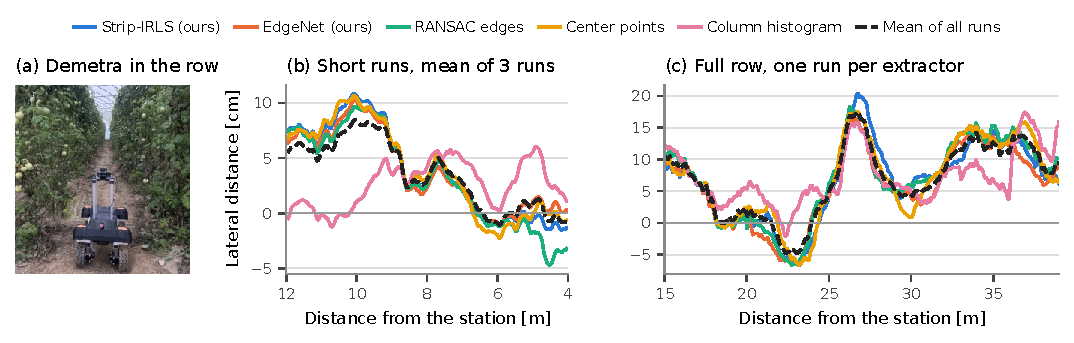
\includegraphics[width=0.9\linewidth]{field_summary.pdf}
  \caption{(a)~Demetra in the tomato row. (b, c)~Lateral distance from the row centerline, with the robot moving from left to right. (b)~Mean of the three short runs of each extractor, at 0.20~m/s. (c)~Full row at 0.50~m/s, one run per extractor. The dashed line is the mean of all the runs.}
  \label{fig:field}
\end{figure}

\section{Conclusions}

Automatic labels, used without correction, can replace manual annotation for the path between parallel rows, with a path IoU about 6 percentage points lower, but not for every class. A network trained only on these labels guided the robot along a tomato row of a field not present in its training data, with each of the five extractors. With EdgeNet, no stage of the chain needs manual annotation. The network learns from automatic labels, and EdgeNet learns from generated masks, has no parameters to set by hand for the extraction and performs like the geometric extractors. Strip-IRLS and EdgeNet have as few gross errors as RANSAC edges and run faster on the Jetson, and with adjacent corridors they also have fewer gross errors. The best extractors fail mostly on the same badly segmented frames, and in the field four of them drove the robot along almost the same trajectory, so the quality of the segmentation affects the result more than the choice among these extractors.

The segmentation was measured against manual masks only on lettuce, with a random split by image, so the results can be optimistic. The field tests cover one row of one crop on one day. A next step is to let the robot navigate the whole greenhouse, whatever the layout of its rows, and not only along one row.

\end{document}
